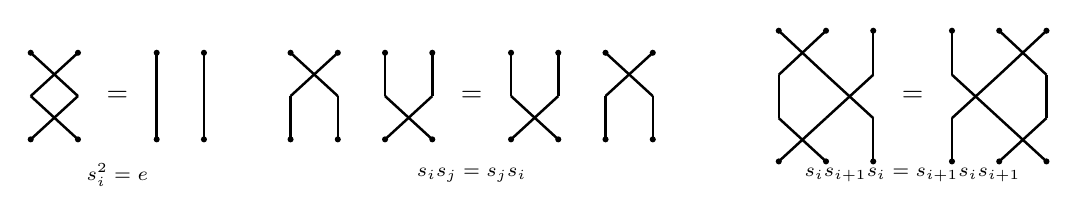
\begin{tikzpicture}[perm/.style={line width=0.9pt}, plab/.style={font=\scriptsize, inner sep=2pt}]
\draw[perm] (0.00,0.00) -- (0.60,-0.55);
\draw[perm] (0.60,0.00) -- (0.00,-0.55);
\draw[perm] (0.00,-0.55) -- (0.60,-1.10);
\draw[perm] (0.60,-0.55) -- (0.00,-1.10);
\fill (0.00,0.00) circle (1.1pt) (0.00,-1.10) circle (1.1pt);
\fill (0.60,0.00) circle (1.1pt) (0.60,-1.10) circle (1.1pt);
\node at (1.10,-0.55) {\(=\)};
\draw[perm] (1.60,0) -- (1.60,-1.10);
\draw[perm] (2.20,0) -- (2.20,-1.10);
\fill (1.60,0.00) circle (1.1pt) (1.60,0.00) circle (1.1pt);
\fill (2.20,0.00) circle (1.1pt) (2.20,0.00) circle (1.1pt);
\fill (1.60,-1.10) circle (1.1pt);
\fill (2.20,-1.10) circle (1.1pt);
\draw[perm] (3.30,0.00) -- (3.90,-0.55);
\draw[perm] (3.90,0.00) -- (3.30,-0.55);
\draw[perm] (4.50,0.00) -- (4.50,-0.55);
\draw[perm] (5.10,0.00) -- (5.10,-0.55);
\draw[perm] (3.30,-0.55) -- (3.30,-1.10);
\draw[perm] (3.90,-0.55) -- (3.90,-1.10);
\draw[perm] (4.50,-0.55) -- (5.10,-1.10);
\draw[perm] (5.10,-0.55) -- (4.50,-1.10);
\fill (3.30,0.00) circle (1.1pt) (3.30,-1.10) circle (1.1pt);
\fill (3.90,0.00) circle (1.1pt) (3.90,-1.10) circle (1.1pt);
\fill (4.50,0.00) circle (1.1pt) (4.50,-1.10) circle (1.1pt);
\fill (5.10,0.00) circle (1.1pt) (5.10,-1.10) circle (1.1pt);
\node at (5.60,-0.55) {\(=\)};
\draw[perm] (6.10,0.00) -- (6.10,-0.55);
\draw[perm] (6.70,0.00) -- (6.70,-0.55);
\draw[perm] (7.30,0.00) -- (7.90,-0.55);
\draw[perm] (7.90,0.00) -- (7.30,-0.55);
\draw[perm] (6.10,-0.55) -- (6.70,-1.10);
\draw[perm] (6.70,-0.55) -- (6.10,-1.10);
\draw[perm] (7.30,-0.55) -- (7.30,-1.10);
\draw[perm] (7.90,-0.55) -- (7.90,-1.10);
\fill (6.10,0.00) circle (1.1pt) (6.10,-1.10) circle (1.1pt);
\fill (6.70,0.00) circle (1.1pt) (6.70,-1.10) circle (1.1pt);
\fill (7.30,0.00) circle (1.1pt) (7.30,-1.10) circle (1.1pt);
\fill (7.90,0.00) circle (1.1pt) (7.90,-1.10) circle (1.1pt);
\draw[perm] (9.50,0.28) -- (10.10,-0.28);
\draw[perm] (10.10,0.28) -- (9.50,-0.28);
\draw[perm] (10.70,0.28) -- (10.70,-0.28);
\draw[perm] (9.50,-0.28) -- (9.50,-0.83);
\draw[perm] (10.10,-0.28) -- (10.70,-0.83);
\draw[perm] (10.70,-0.28) -- (10.10,-0.83);
\draw[perm] (9.50,-0.83) -- (10.10,-1.38);
\draw[perm] (10.10,-0.83) -- (9.50,-1.38);
\draw[perm] (10.70,-0.83) -- (10.70,-1.38);
\fill (9.50,0.28) circle (1.1pt) (9.50,-1.38) circle (1.1pt);
\fill (10.10,0.28) circle (1.1pt) (10.10,-1.38) circle (1.1pt);
\fill (10.70,0.28) circle (1.1pt) (10.70,-1.38) circle (1.1pt);
\node at (11.20,-0.55) {\(=\)};
\draw[perm] (11.70,0.28) -- (11.70,-0.28);
\draw[perm] (12.30,0.28) -- (12.90,-0.28);
\draw[perm] (12.90,0.28) -- (12.30,-0.28);
\draw[perm] (11.70,-0.28) -- (12.30,-0.83);
\draw[perm] (12.30,-0.28) -- (11.70,-0.83);
\draw[perm] (12.90,-0.28) -- (12.90,-0.83);
\draw[perm] (11.70,-0.83) -- (11.70,-1.38);
\draw[perm] (12.30,-0.83) -- (12.90,-1.38);
\draw[perm] (12.90,-0.83) -- (12.30,-1.38);
\fill (11.70,0.28) circle (1.1pt) (11.70,-1.38) circle (1.1pt);
\fill (12.30,0.28) circle (1.1pt) (12.30,-1.38) circle (1.1pt);
\fill (12.90,0.28) circle (1.1pt) (12.90,-1.38) circle (1.1pt);
\node[font=\scriptsize] at (1.1,-1.55) {\(s_i^2 = e\)};
\node[font=\scriptsize] at (5.6,-1.55) {\(s_i s_j = s_j s_i\)};
\node[font=\scriptsize] at (11.2,-1.55) {\(s_i s_{i+1} s_i = s_{i+1} s_i s_{i+1}\)};
\end{tikzpicture}
